\apendice{Plan de Proyecto Software}

\section{Introducción}

Ojo \footnote{Los anexos deben de tener su propia bibliografía, eso es tan fácil como utilizar referencias igual que en la memoria \cite{bortolot2005}}

\section{Planificación temporal}
% Inicio de la figura
\begin{figure}[h]
    \centering
    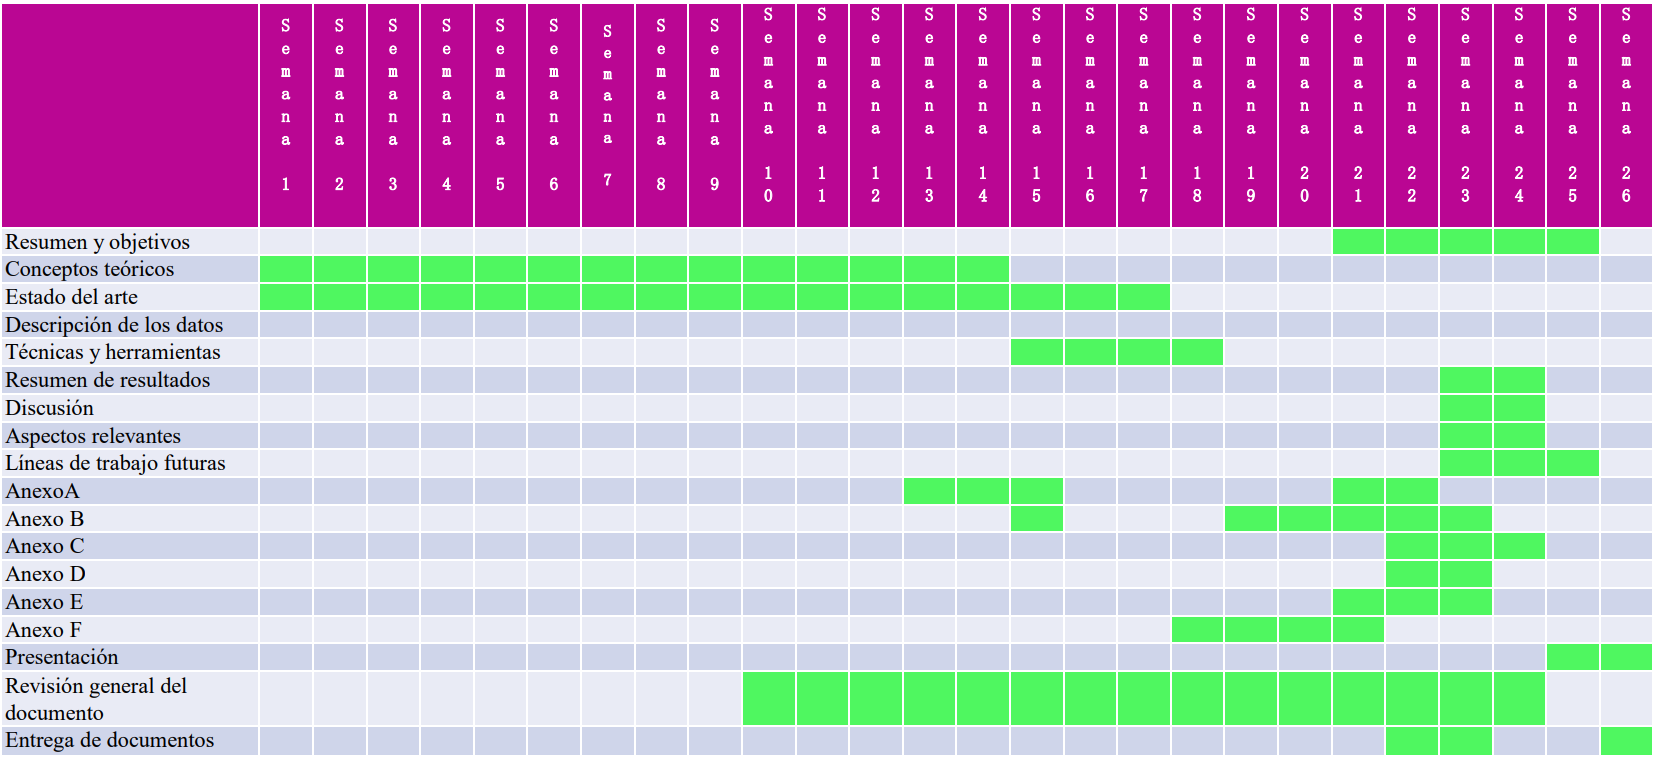
\includegraphics[width=1\textwidth]{img/PlanificacionTemporal.png}
    \caption{Planificación temporal seguida para la realización de este proyecto.}
    \label{fig:planTemporal} % Esta etiqueta es la que permite que se encuentr referenciada en el texto (es muy importante que siempre estén referenciadas en el texto)
\end{figure}
% Añadir una imagen con los hitos por semanas unas 14 semanas aprox aunque puede variar en funcion se vaya avanzando, en cuyo caso se volverá a modificar la tabla

\section{Planificación económica}
Para obtener una buena planificación económica se deberán identificar los gastos y los ingresos relacionados con el desarrollo del producto.

Como primeros gastos incluiremos el precio de los componentes y los gastos de producción, mientras que para obtener los ingresos se tendrá en cuenta el beneficio, gastos imprevistos e I+D del producto, para posibles mejoras en e futuro. La suma de gastos e ingresos nos devolverá el precio final del dispositivo.


% ----------------------------------------------------
% Tabla del desglose económico de las versiones realizadas.
\begin{table}[h!]
\centering
\begin{tabular}{ |m{4cm}|m{4cm}|m{2cm}|m{2cm}|  } 
\hline
\cellcolor[HTML]{B9E3F0}\textbf{} & \cellcolor[HTML]{B9E3F0}\textbf{Cálculos} & \cellcolor[HTML]{B9E3F0}\textbf{Versión 1}& \cellcolor[HTML]{B9E3F0}\textbf{Versión 2}\\

\hline
\cellcolor[HTML]{EFEFEF}\textbf{Gastos de los componentes}             & {Suma de los precios de cada componente del producto}   & 27€ & 32.5€\\
\hline
\cellcolor[HTML]{EFEFEF}\textbf{Gastos de producción}                & {10\% del precio de los componentes} & 2.7€ & 3.25€\\
\hline
\cellcolor[HTML]{EFEFEF}\textbf{Ingresos destinados a beneficio}                & {5\% del total de gastos} & 1.48€ & 1.79€\\
\hline
\cellcolor[HTML]{EFEFEF}\textbf{Gastos imprevistos e I+D} & {10\% del total de gastos} & 2.97€ & 3.58€\\
\hline
\cellcolor[HTML]{EFEFEF}\textbf{Precio Total} & {Suma de los gastos e ingresos} & \textbf{34.15€} & \textbf{41.10€}\\
\hline
\end{tabular}
\caption{Resumen de gastos y precio total del producto}
\end{table}

El prototipo de la versión 1, en la que se emplea el sensor SW520D, tiene un coste final aproximado\footnote{La planificación económica será variable en el tiempo y durante el desarrollo del producto, por lo que se trata de precios totales aproximados. Igual para el prototipo versión 2.} de unos 34.15€, precio que podría ser menor al crear nuestro propio microcontrolador o utilizar una alternativa similar a arduino, puesto que es el elemento que más aumenta el precio de la solución, siendo el precio del resto de los componentes aproximadamente unos 3€.

El prototipo de la versión 2, en la que se emplea el sensor SW520D, tiene un coste final aproximado de unos 41.10€, precio que también podría disminuir al crear nuestro propio microcontrolador o utilizar una alternativa a arduino, ya que sin el microcontrolador Arduino el precio ronda los 8.5€.


\subsection{Desglose de los precios de los componentes del prototipo Versión 1}

Se han tenido en cuenta los precios más bajos encontrados de cada componente necesario.
%\usepackage{siunitx}
\begin{itemize}
    \item Arduino UNO R3: 24€
    \item Resitencias (330 \textOmega, 2x220 \textOmega, 33 \textOmega, 1000 \textOmega): 0.05€
    \item Zumbador pasivo: 0.25€
    \item Motor de vibración: 1€
    \item Transistor: 0.05€
    \item SW520D: 0.5€
    \item Led azul: 0.02€
    \item Pulsador: 0.05€
    \item Otros elementos variados: 1€
    
\end{itemize}

\subsection{Desglose de los precios de los componentes del prototipo Versión 2}

Se han tenido en cuenta los precios más bajos encontrados de cada componente necesario.
%\usepackage{siunitx}
\begin{itemize}
    \item Arduino UNO R3: 24€
    \item Resitencias (2x330 \textOmega, 2x220 \textOmega, 33 \textOmega, 1000 \textOmega): 0.06€
    \item Zumbador pasivo: 0.25€
    \item Motor de vibración: 1€
    \item Transistor NPN: 0.05€
    \item MPU-6050: 6€
    \item Led azul: 0.02€
    \item 2xPulsador: 0.10€
    \item Otros elementos variados: 1€
    
\end{itemize}




\section{Viabilidad legal}

Respecto a la viabilidad legal es respecto a que partes del desarrollo o comercialización  pueden pararse por problemas legales.

Datos almacenados de los usuarios.

Incluir que debe cumplir con la ley de protección de datos...

Si el dispositivo se llegase a crear y se pudiera sacar a mercado deberá cumplir con los requisitos legales de dispositivos médicos que garantice en todo momento la protección de los usuarios a los que está enfocado el dispositivos. Alguna de las leyes que se deberán tener en cuenta son:
\begin{itemize}
    %\item Directiva 2014/35/UE del Parlamento Europeo y del Consejo aprobada el 26 de febrero de 2014 sobre la armonización de las legislaciones de los Estados miembros en materia de comercialización  de material eléctrico destinado a utilizarse con determinados límites de tensión. % fuera porque este dispositivo utiliza poca corriente. esta directiva está dirigida a dispositivos que emplean una tensión comprendida entre 50 y 1000 V en corriente alterna y entre 75 y 1500 V en corriente continua.
    % https://www.boe.es/doue/2014/096/L00357-00374.pdf
    \item Directiva 2014/30/UE aprobada el 26 de febrero de 2014 aprobada por el Parlamento Europeo y el Consejo sobre la armonización de las legislaciones de los Estados miembros en materia de compatibilidad electromagnética (refundición). Establece que los dispositivos electrónicos que se comercializan en Europa cumplan con los requisitos de compatibilidad electromagnética.
    % https://www.boe.es/doue/2014/096/L00079-00106.pdf
    \item Ley Orgánica 3/2018, de 5 de diciembre, de Protección de Datos Personales y garantía de los derechos digitales. Para poder proteger cualquier información que identifique a una persona, de forma confidencial. Además, el usuario debe estar correctamente informado del tratamiento de sus datos, ademas el acceso al tratamiento de sus datos debe ser claro y accesible.

    El usuario tendrá derecho al acceso de sus datos, derecho de rectificación y supresión de sus datos, derecho a la limitación del tratamiento de sus datos, derecho a la portabilidad de sus datos y el derecho a oponerse al tratamiento de sus datos. Por todo ello el tratamiento de sus datos debe ser tras la confirmación clara del consentimiento informado del tratamiento de sus datos.
    
    \item Reglamento UE 2016/679 relativo a Protección de las Personas Físicas en lo que respecta al tratamiento de datos personales y circulación de estos Datos. Donde se define que se debe garantizar la protección de los datos con los que se trabaja, además de notificar brechas de seguridad o exposición de datos al usuario.

    \item Ley 21/2014, de 4 de noviembre, por la que se modifica el texto refundido de la Ley de Propiedad Intelectual 

    \item La Ley 34/2.002 de Servicios de la Sociedad de la Información y de Comercio Electrónico, en caso de que se realice una tienda web oficial de comercialización del dispositivo.
    \item La Ley 56/2007 de 28 de Diciembre, de Medidas de Impulso de la Sociedad de la Información 

    \item Ley 24/2015, Ley de Patentes, donde se regula todo lo relacionado con invenciones empleando patentes.
    % Referencia: 
    % https://www.boe.es/buscar/act.php?id=BOE-A-2015-8328
    
    \item Además, se debera tener en cuenta la Ley 7/1996, de 15 de enero, de Ordenación del Comercio Minorista.
    
    \item normativa de sanidad
    
    \item Normativa laboral
    \item Normativa de fases de prueba.
    \item En función de los problemas que pueden surgir... Dividir en 3 fases, creación de la idea, diseño y desarrollo y producción de pruebas, venta y posventa(demandas y gestion de los datos). Se debe tener en cuenta que el dispositivo tenga un funcionamiento seguro que no afecte negativamente al usuario.
    
\end{itemize}

Además el dispositivo deberá contar con un certificado CE, que garantizará que el dispositivo cumple con los requisitos de seguridad, protección y sanidad europeos. Una vez se obtenga el certificado el dispositivo podrá ser comercializado legalmente en la Unión Europea.
% Referencia:
%https://europa.eu/youreurope/business/product-requirements/labels-markings/ce-marking/index_es.htm